\documentclass[a4paper, 12pt]{article}
\usepackage{cmap}
\usepackage{amssymb}
\usepackage{amsmath}
\usepackage{graphicx}
\usepackage{amsthm}
\usepackage{upgreek}
\usepackage{setspace}
\usepackage[T2A]{fontenc}
\usepackage[utf8]{inputenc}
\usepackage[normalem]{ulem}
\usepackage{mathtext} % русские буквы в формулах
\usepackage[left=2cm,right=2cm, top=2cm,bottom=2cm,bindingoffset=0cm]{geometry}
\usepackage[english,russian]{babel}
\newenvironment{Proof} % имя окружения
{\par\noindent{}} % команды для \begin
{\hfill$\scriptstyle$}
\newcommand{\Rm}{\mathbb{R}}
\newcommand{\Cm}{\mathbb{C}}
\newcommand{\I}{\mathbb{I}}
\newcommand{\N}{\mathbb{N}}
\newcommand{\Sp}{\text{Sp}}
\newtheorem*{theorem}{Теорема}
\newtheorem*{cor}{Следствие}
\renewcommand{\epsilon}{\upvarepsilon}
\newcommand\Norm[1]{\left\| #1 \right\|}
\newtheorem*{lem}{Лемма}
\newcommand{\FI}{\text{Ф}}
\renewcommand{\tau}{\uptau}
\newcommand{\Ln}{L_n = D^n + a_{n-1}D^{n-1} + \ldots + a_1D + a_0D^0}
\begin{document}
	\section*{Фазовая плоскость СтЛВУ. Классификация точек покоя.}
	Рассмотрим уравнение $$DX = AX,\eqno(1)$$ где $$A = \begin{pmatrix}
		a & b \\ c & d
	\end{pmatrix},\text{ а } X(t) = \begin{pmatrix}
		x_1(t)\\x_2(t)
	\end{pmatrix}$$ --- неизвестная векторная функция.\\\\
	$\bullet$ \textit{\textbf{Фазовым графиком} решения $X(t)$ называется график функции} $$\begin{cases}
		x_1 = x_1(t),\\
		x_2 = x_2(t).
	\end{cases}$$
	$\bullet$\textit{ Плоскость $Ox_1x_2$, на которой располагаются фазовые графики решений, называется \textbf{фазовой плоскостью уравнения}.}\\\\
	$\bullet$ \textit{Фазовый график, состоящий из одной точки, называется \textbf{точкой покоя}}.\\\\
	Начало координат (точка (0; 0)) всегда является точкой покоя для уравнения (1). Рассмотрим классифицкации точек покоя.\\\\
	\textbf{I группа.} \begin{enumerate}
		\item Пусть матрица $A = \begin{pmatrix}
			0 & 0\\
			0 & 0
		\end{pmatrix}$. Тогда любая точка фазовой плоскости является фазовым графиком и других фазовых графиков нет.
		\item Пусть $A = aE$, то есть $A = \begin{pmatrix}
			a & 0\\
			0 & a
		\end{pmatrix}$.\\\\
	$\bullet$ \textit{Точка покоя, в окрестности которой фазвоые графики имеют такое расположение, называется \textbf{дикритическим узлом} причем при $a > 0$ \textbf{устойчивым}, а при $a<0$ \textbf{неустойчивым}.}
	\end{enumerate}
	\textbf{II группа.} Пусть $A = \begin{pmatrix}
		a & b\\c & d
	\end{pmatrix}$, причем $A \ne aE$. Рассмотрим матрицу $B = \begin{pmatrix}
		0 & 1\\
		-\det A & \Sp A
	\end{pmatrix}$, $\Sp A = a+d$. Матрицы $A$ и $B$ подобны, то есть $\exists S, \det S \ne 0 : B = S^{-1}AS.$\\\\
	Выполним замену в уравнении (1) неизвестной функции $X = SY$. Тогда $$DY = BY.\eqno(2)$$
	Координатная форма уравнения (2) имеет вид $$\begin{cases}
		Dy_1 = y_2,\\
		Dy_2 = -\det A y_1 + \Sp A Dy_1.
	\end{cases}$$ Исключим из второго уравнения $y_1$ и получим $$D^2y_1 - (\Sp A)Dy_1 + (\det A)y_1 = 0.$$
	Тогда решение $y_1(t)$ имеет фазовую тракекторию, являющуюся графиком функции $$\begin{cases}
		y_1 = y_1(t),\\
		y_2 = Dy_1(t);
	\end{cases}\Rightarrow \begin{cases}
		y_1 = y_1(t),\\
		y_2 = y_2(t).
	\end{cases}\eqno(3)$$
	Типы точек покоя уравнения (1) будут совпадать с типами точек покоя уравнений (2) и (3). То есть все остальные классификации точек покоя мы можем перенести с СтЛУ на СтЛВУ.\\\\ Пусть $\lambda_1$, $\lambda_2$ --- корни характеристического уравнения $\lambda^2 + a_1\lambda + a_0 = 0$ для уравнения (1). Тогда тип точки покоя $O$ при $a_0 \ne 0$ определяется следующим образом:\begin{enumerate}
		\item Если $\lambda_1$, $\lambda_2$ $\in \Rm$ и
		\begin{enumerate}
			\item $\lambda_1\cdot \lambda_2 < 0$, то точка покоя называется \textbf{седлом};
			\item $\lambda_1\cdot \lambda_2 > 0$, $\lambda_1 \ne \lambda_2$, то точка покоя называется \textbf{бикритическим узлом}, причем, при $\lambda_1 < \lambda_2 < 0$ \textbf{устойчивым}; при $\lambda_2 > \lambda_1 > 0$ \textbf{неустойчивым};
			\item $\lambda_1\cdot \lambda_2 > 0$, $\lambda_1 = \lambda_2$, то точка покоя называется \textbf{монокритическим узлом}, причем, при $\lambda_1 = \lambda_2 < 0$ \textbf{устойчивым}; при $\lambda_2 = \lambda_1 > 0$ \textbf{неустойчивым};
		\end{enumerate}
		\item Если $\lambda_{1,2} = \alpha \pm \beta i$ и\begin{enumerate}
			\item $\alpha \ne 0$, $\beta \ne 0$, то точка покоя называется \textbf{фокусом}, причем, при $\alpha < 0$ \textbf{устойчивым}; при $\alpha > 0$ \textbf{неустойчивым};
			\item $\alpha = 0$, $\beta \ne 0$, то точка покоя называется \textbf{центром}.
		\end{enumerate}
	\end{enumerate}
	Если характеристическое уравнение имеет вид $\lambda^2 + a_1\lambda = 0$, где $a_1 \geqslant 0$, то прямая $x_1 = x_2$ состоит из точек покоя и называется \textbf{прямой покоя}.\\\\
	Исследование типа точки покоя проводится аналогично исследованию в СтЛУ.\\\\
	\textbf{Пример 1.} Установить тип точки покоя для уравнения $DX = AX$, где $$A = \begin{pmatrix}
		3 & 1\\
		1 & 3
	\end{pmatrix}.$$
\textbf{Решение.} Построим характеристическое уравнение и найдем его корни:
$$\det (A - \lambda E) = \begin{vmatrix}
	3 - \lambda & 1\\
	1 & 3 - \lambda
\end{vmatrix} = \lambda^2 - 6\lambda + 8 = (\lambda - 2)(\lambda - 4) = 0.$$ Корни уравнения $\lambda_1 = 2$, $\lambda_2 = 4$. Тогда точка $O$ является неустойчивым бикритическим узлом.\\\\
\textbf{Ответ:} Точка $O$ --- неустойчивый бикритический узел.\\\\
\textbf{Пример 2.} Установить тип точки покоя для уравнения $DX = AX$, где $$A = \begin{pmatrix}
	-5 & 0\\
	0 & -5
\end{pmatrix}.$$
\textbf{Решение.} Матрица $A = (-5)E$, то есть ее вид совпадает с видом матрицы $A$ для случая, когда точка $O$ является дикритическим узлом, причем устойчивым, так как коэффициент $a$ отрицательный.\\\\ 
\textbf{Ответ:} Точка $O$ --- устойчивый дикритический узел.\\\\
Аналогичным образом рассматриваются и параметрические уравнения.\\\\
\textbf{Пример 3.} Определить тип точки покоя для уравнения $DX = AX$, где $$A = \begin{pmatrix}
	-3\alpha & 1\\
	-3 & 0
\end{pmatrix}.$$ в зависимости от значений параметра $\alpha$.\\\\
\textbf{Решение.} Построим характеристическое уравнение:
$$\det(A - \lambda E)  = \begin{vmatrix}
	-3\alpha - \lambda & 1\\
	-3 & -\lambda
\end{vmatrix} = \lambda^2 + 3\alpha\lambda + 3 = 0.$$
Тогда корни уравнения имеют вид $$\lambda_1 = \dfrac{-3\alpha + \sqrt{9\alpha^2 - 12}}{2},\quad \lambda_2 = \dfrac{-3\alpha - \sqrt{9\alpha^2 - 12}}{2}.$$\begin{enumerate}
	\item Пусть $9\alpha^2 - 12 > 0$. Тогда $|\alpha| > \dfrac{2}{\sqrt{3}}$. Подставим $\alpha$ в $\lambda_1$ и $\lambda_2$ и получим $\lambda_1, \lambda_2 \in \Rm$, $\lambda_1 \ne \lambda_2$, $$\lambda_1 \cdot \lambda_2 = \dfrac{9\alpha^2 - 9\alpha^2 + 12}{4} = 3 > 0,$$ следовательно, точка $O$ --- бикритический узел. Причем при $\alpha > \dfrac{2}{\sqrt{3}}$ получаем устойчивый бикритический узел, а при $\alpha < -\dfrac{2}{\sqrt{3}}$ --- неустойчивый.
	\item Пусть $9\alpha^2 - 12 = 0$. Тогда $|\alpha| = \dfrac{2}{\sqrt{3}}$. Подставим $\alpha$ в $\lambda_1$ и $\lambda_2$ и получим $\lambda_1, \lambda_2 \in \Rm$, $\lambda_1 = \lambda_2 = -\dfrac{3}{2}$, $\lambda_1\cdot\lambda_2 > 0$. Таким образом, точка $O$ --- монокритический узел. Причем при $\alpha = \dfrac{2}{\sqrt{3}}$ получаем устойчивый бикритический узел, а при $\alpha = -\dfrac{2}{\sqrt{3}}$ --- неустойчивый.
	\item Пусть $9\alpha^2 - 12 < 0$. Тогда получаем два случая:\begin{enumerate}
		\item $0 < |\alpha| < \dfrac{2}{\sqrt{3}}$. Таким образом, $\lambda_{1,2} = \alpha \pm \beta i$ и $\alpha \ne 0$. Тогда точка $O$ --- фокус, причем при $0 <\alpha < \dfrac{2}{\sqrt{3}}$ устойчивый, а при  $0 > \alpha >- \dfrac{2}{\sqrt{3}}$ неустойчивый.
		\item $\alpha = 0$. Таким образом, $\lambda_{1,2} = \pm \beta i$, и точка $O$ --- центр.
	\end{enumerate}
\end{enumerate}
\textbf{Пример 4.} Установить тип точки покоя и начертить фазовый портрет для уравнения $DX = AX$, где $$A = \begin{pmatrix}
	-2 & -4\\
	-1 & 1
\end{pmatrix}.$$
\textbf{Решение.} Для начала необходимо установить тип точки покоя для данного уравнения. Построим характеристическое уравнение и найдем его корни:
$$\det(A - \lambda E) = \lambda^2 + \lambda - 6 = (\lambda +3)(\lambda -2 ) = 0.$$ То есть корни данного характеристического уравнения $\lambda_1 = -3$, $\lambda_2 = 2$. Таким образом, точка $O$ --- седло. То есть построенный в итоге график будет соответствовать виду фазового графика такой точки покоя. Теперь построим матрицу $$B = \begin{pmatrix}
	0 & 1\\
	-\det A & \Sp A
\end{pmatrix} = \begin{pmatrix}
0 & 1\\
6 & -1
\end{pmatrix},$$ которая является подобной матрице $A$, то есть $\exists S, \det S \ne 0 : B = S^{-1}AS.$ Выполним замену $X = SY$ для исходного уравнения и получим уравнение вида $$DY = BY\Longleftrightarrow\begin{cases}
Dy_1 = y_2,\\
Dy_2 = 6y_1 - Dy_1.
\end{cases}$$
Исключим $y_1$ из второго уравнения и получим СтЛОУ $$D^2y_1 + Dy_1 - 6y_1 = 0.$$ Фазовый портрет такого уравнения мы уже умеем строить, и задается он параметрически заданной функцией $$\begin{cases}
	y_1 = y_1(t),\\
	y_2 = Dy_1(t).
\end{cases}$$
Полученное СтЛОУ имеет корни $\lambda_1 = -3$, $\lambda_2 = 2$. Следовательно, $y_1(t) = C_1e^{-3t} + C_2e^{2t}$. Подставим $y_1(t)$ и $Dy_1(t)$ в параметрическое уравнение и получим, что фазовый портрет СтЛОУ задается системой $$\begin{cases}
	y_1 = C_1e^{-3t} + C_2e^{2t},\\
	y_2 = -3C_1e^{-3t} + 2C_2e^{2t}.
\end{cases}$$
Мы уже знаем, каким уравнением задается фазовый портрет и какой вид он имеет (седло). Остается выяснить асимптоты, к которым стремятся фазовые графики. Для этого найдем пределы 
$$\lim\limits_{t\to+\infty} \dfrac{y_2(t)}{y_1(t)}=\dfrac{-3C_1e^{-3t} + 2C_2e^{2t}}{ C_1e^{-3t} + C_2e^{2t}} = 2.$$
$$\lim\limits_{t\to-\infty} \dfrac{y_2(t)}{y_1(t)}=\dfrac{-3C_1e^{-3t} + 2C_2e^{2t}}{ C_1e^{-3t} + C_2e^{2t}} = -3.$$
Таким образом, прямые $y_2 = 2y_1$ и $y_2 = -3y_1$ являются асимптотами фазовых графиков. А в точках, где $Dy_2 = 0$, то есть $-a_1y_2 - a_0y_1 = 0$, то есть на прямой $y_2 = 6y_1$ касатлельные к фазовым графикам параллельны оси $Ox$ (т.е. на пересечении с этой прямой у верхних и нижних графиков находится точка перегиба). Построим фазовый портрет на основании полученной информации: (см. следующую страницу)\\\\
Однако полученный фазовый портрет соответствует лишь уравнению $DY = BY$, но не исходному. Для получения фазового портрета исходного уравнения сделаем обратное линейное преобразование $X = SY$, где $S$ --- матрица перехода от базиса $A$ к базису $B$ 
\\
$$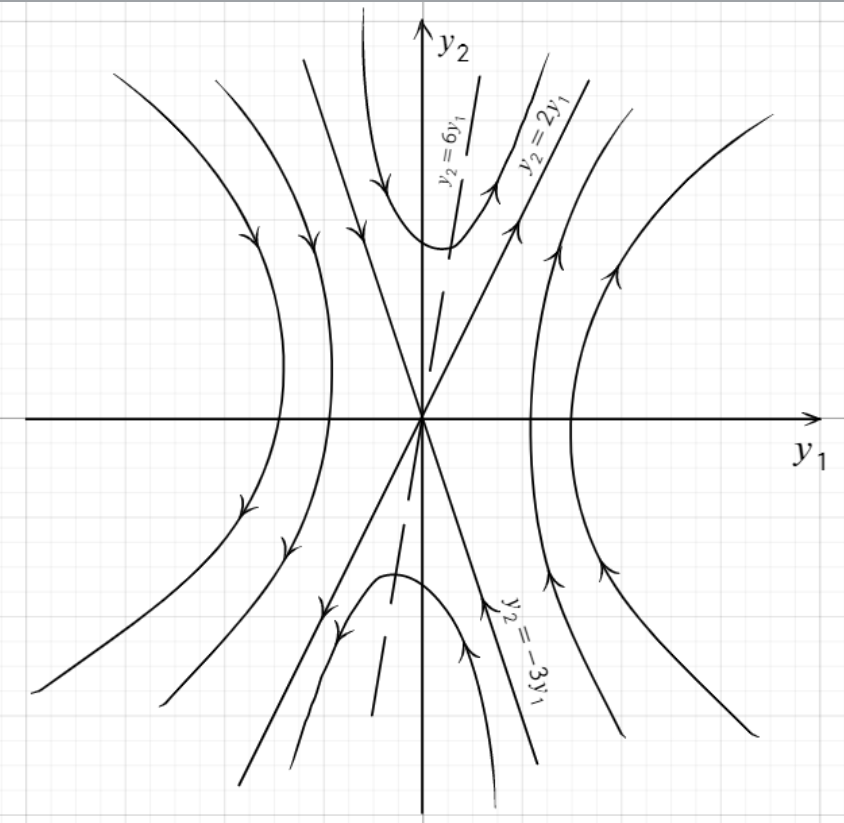
\includegraphics[scale=0.8]{images/stlvu_gr_1.png}$$
\end{document}